\documentclass{article}
\usepackage[utf8]{inputenc}
\usepackage{graphicx}
\usepackage{fancyhdr}
\usepackage{geometry}
\usepackage{amsmath}
\usepackage{amssymb}
\usepackage{array}
\usepackage{url}
\usepackage{hyperref}
\usepackage{subcaption}

\geometry{left = 2cm, right=2cm, bottom=2cm, top=2cm}

\title{3806ICT - Maze Planning and Replanning with Reinforcement Learning}
\author{Zac Jensen - s5153515 - zac.jensen@griffithuni.edu.au \\
    Jake Muggleton - s5130398 - jake.muggleton@griffithuni.edu.au}

\pagestyle{fancy}
\renewcommand{\headrulewidth}{1pt}
\fancyhf{}
\rhead{3806ICT - Maze Solving}
\chead{Griffith University}
\lhead{}
\rfoot{Page \thepage}
\newcommand\tab[1][1cm]{\hspace*{#1}}

\begin{document}
    \maketitle

%==============================================================================

    \section{Abstract}\label{sec:abstract}
        This report explores the problem of autonomous agent planning and replanning in a dynamic environment. In this report, an agent uses Q-learning (reinforcement learning) to navigate through a 2D grid-maze environment towards a goal position. During its navigation however, obstacles in the environment, and the goal position may change. The agent uses replanning techniques to navigate this dynamic environment to successfully reach the goal. A model for such a scenario is presented which is then tested for mazes of various sizes. In most cases, the agent is able to successfully navigate the dynamic environment towards the goal. 

    \section{Introduction}\label{sec:introduction}
        A maze world is defined as a 2D matrix of ASCII characters where ‘O’ is an open cell that the agent can step to, ‘H’ is a closed wall that the agent cannot step to, ‘G’ is the goal position for the agent, and ‘S’ is the start position for the agent. The agent may move around the maze by taking ‘steps’, where each step may involve moving up,down,left, or right by one cell. In this report, first a model representing an agent navigating a static (unchanging) maze world is shown. Next, a method for creating a dynamic environment is proposed. Finally, experiments on this model are conducted and an analysis of the results is performed.

    \section{Planning in a Static Environment}\label{sec:test-design}
        To model an agent navigating a static environment, a maze generation program aswell as a Q-learning based Reinforcement Learning (RL) algorithm were used which are available from the supplied ‘2021-assignment-sample2’ folder [1]. This model is available as ‘GridWorld-task2.py’ and can be run using the command line ‘python3 GridWorld-task2.py [maze\_width] [maze\_height]’.

In this model, a maze is randomly generated with a start point and goal point using a common random depth-first search (DFS) based algorithm. The Q-learning algorithm then provides a set of steps (a trace) towards the goal from the start. An extra constraint for this model is that the agent can take no more than 2N steps where N is the width of the NxN maze. 

The model is outlined in the following pseudocode:\\
\hspace*{4cm}maze $\leftarrow$ generateMaze(height, width)\\
\hspace*{4cm}RLSolver $\leftarrow$ initialise Q-Learning solver\\
\hspace*{4cm}trace $\leftarrow$ RLSolver.solve(maze)\\
\hspace*{4cm}if trace.length $<$ 2*width:\\
\hspace*{5cm}goal $\leftarrow$ reached


\section{Programming A Dynamic Environment}\label{sec:test-design}
	To model a dynamic environment, a function was created which takes an existing maze and returns a new maze which is a ‘mutation’ of the original. This model is available as ‘GridWorld-task3.py’ which calls mutate\_maze() in ‘MutateMaze.py’ and can be run using the command line ‘python3 GridWorld-task3.py [maze\_width] [maze\_height]’. 

	The constraints for this are that the new maze must share similarities to the old one, and obstacles in the new maze mustn’t overlap with the current, or previous positions of the agent. The goal must also not be blocked off from the agent by obstacles. To generate a mutation, first all of the previous positions of the agent are collected. Next, multiple random walks are conducted from the agents current position in the original maze, keeping track of all cells visited by the search. A new maze is initialised with all of the agent’s previous positions and cells visited by the random walks and the DFS maze generation algorithm is run to generate a new maze containing these cells. Finally, the new goal location is set using a random walk, where the walk becomes shorter if the agent has taken alot of steps. This mutation method generates a new maze that guarantees that the goal is reachable and the agent or its previous positions are not overlapped by an obstacle. It also produces a maze that has a similar structure to the old maze for all cells close to the agent, but becomes increasingly different for cells further away from the agent. 

	The model is demonstrated by using the model from task 2, and then mutating the maze once the agent reaches the goal. Figure 1 shows the three steps involved in a maze mutation including the original maze, initialising the new maze with the previous positions of the agent aswell as the paths of multiple random walks, and finally the newly generated maze. Here, ‘u’ is a maze element which hasn’t yet been initialised. 

\begin{figure}[ht]
	\centering
	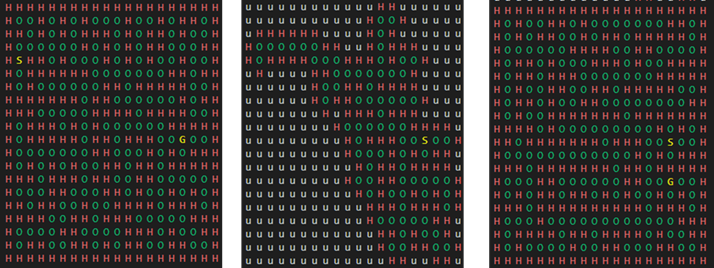
\includegraphics[width=\textwidth]{assets/mutateMaze.png}
	\caption{The Three Steps of A Maze Mutation. Initial Maze (Left), Choosing Maze Features To Keep (Middle), Mutated Maze (Right)}
\end{figure}


\section{Replanning in a Dynamic Environment}\label{sec:test-design}

	To model planning and replanning in a dynamic environment, the agent in task 2 and the mutation function in task 3 were combined. This model is available as ‘GridWorld-task4.py’ and can be run using the command line ‘python3 GridWorld-task4.py [maze\_width] [maze\_height]’.

Here, after calling the program on the command line, an initial maze is generated. The agent then autonomously plans a route towards the goal and starts taking steps towards it. At each step there is a 10\% chance that the maze mutates. If so, the maze is mutated with the function created in task 3. The agent then replans its route by solving the maze from its current position. Finally, the program terminates when either the agent reaches the goal, or the agent has taken more than 2*width steps, in which case the agent is reported to have failed. \\

The model is outlined in the following pseudocode:\\
\hspace*{2cm}maze $\leftarrow$ generateMaze(height, width)\\
\hspace*{2cm}agent $\leftarrow$ agent object positioned at maze.start\\
\hspace*{2cm}steps $\leftarrow$ empty list\\
\hspace*{2cm}while agent has not reached goal and steps.size $<$ 2*width\\
\hspace*{3cm}trace $\leftarrow$ RLSolver.solve(maze)\\
\hspace*{3cm}for step in trace:\\
	\hspace*{4cm}steps.append(step)\\
	\hspace*{4cm}agent $\leftarrow$ update agent position to step\\
	\hspace*{4cm}if 10\% chance occurs: mutate maze and break from for loop\\
\hspace*{2cm}check if agent at goal

\begin{figure}[ht]
	\centering
	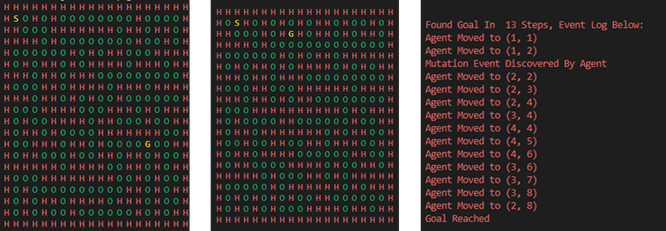
\includegraphics[width=\textwidth]{assets/task4figure.png}
	\caption{Original Maze (Left), Mutated Maze (Mid), and Agent Log (Right)}
\end{figure}

Figure 2 shows a 20x20 maze example of the agent planning-replanning model, including the original maze, a mutation that occurs, and the agent's movements throughout the process. The agent can be seen to alter its course towards the new goal once it discovers a mutation event.


\section{Experimentation }\label{sec:experimentation} 
To assess the performance of the replanning model, an experiment was carried out. For maze sizes of 10x10, 50x50, and 100x100, the algorithm from task 4 was run 10 times each. The performance of the algorithm was then recorded, with the results presented in table 1 below. In terms of hardware, the experiment was performed using Python inside Visual Studio Code, on a Windows 10 PC with a Ryzen 5 3600 and 32GB of RAM. The parameters of the Reinforcement Learning Agent were set to gamma=0.99, alpha=0.1, epsilon=0.1, max iterations=3000, and max steps=1000.


    \section{Results}\label{sec:results}

        \begin{tabular}{ | m{1cm} | m{5em}| m{2cm} | m{2cm} | m{2cm} | m{2cm} | m{2cm} | m{2cm} | } 
	\hline
	Size & Number of Times Goal was reached & Minimum Path Length & Maximum Path Length & Average Path Length & Average time taken
	per maze (s) & Average number of Mutations & Total time taken (s)\\
	  \hline
	  10 & 10 & 2 & 18 & 10 & 1.26 & 0.6 & 12.61 \\ 
	  \hline
	  50 & 10 & 19 & 59 & 38.5 & 46.49 & 3.7 & 464.87 \\ 
	  \hline
	  100 & 10 & 10 & 99 & 53.8 & 99.6 & 5.4 & 996.7 \\ 
	  \hline
	\end{tabular}
	Table 1: Aggregate results for task 4 (n=10 iterations per size).
	\vspace*{1cm} \\
	As can be seen from the table above, in all 30 maze trials, a goal was successfully reached within 2*N moves. The table also shows some more interesting information, such as the minimum, maximum and average path length, the average time taken per maze, the average number of mutations, and the total time required to solve the 10 trials for each separate size. The difference in results between the mazes of size 10 and 50 are greater than the expected 5 times increase. Although, the difference between the size 50 and size 100 mazes is approximately doubled for all results, as would be expected from that size increase. Interestingly though, the minimum path length found for the size 100 mazes was almost half that of the size 50 maze, likely due to the randomness of the maze generation.

    
	\section{Conclusion}\label{sec:conclusion}
	This report shows that given a dynamic environment, to achieve its goal, an agent must be able to perform a planning-replanning cycle. Presented in this report is a model for such an agent based on Q-learning as well as a method for creating a dynamic environment for a 2D maze world based on the DFS maze generation algorithm. For future experiments, it is advised that the Q-learning algorithm may converge more quickly if its Q-table is kept after each mutation rather than being initialised to zeros each time. This would allow for less training iterations and therefore better performance in terms of time. 

	\section{References}\label{sec:references}
	[1] 2021-assignment-sample2 (2021), Publisher Unknown, Accessed 18/06/2022, Made Available Through Grifith University. 
https://bblearn.griffith.edu.au/bbcswebdav/pid-6854529-dt-content-rid-123669136\_1/xid-123669136\_1 

%==============================================================================
    \bibliographystyle{apalike}
    \bibliography{biblio}
\end{document}
